The main contribution of this thesis is represented by the design of a toolchain for Graph Neural Network acceleration on FPGA leveraging High-Level Synthesis.

This chapter explains in detail how the toolchain has been designed and how it can be used to build GNN accelerators to enhance inference performance.

The core component of the toolchain is the synthesizer, enclosing SODA-OPT~\cite{9786533} and PandA-Bambu~\cite{9586110}.
The primary objective of this thesis is to enhance SODA-OPT and PandA-Bambu to synthesize GNN models written in high-level frameworks, such as PyTorch, to FPGA architectures.

Figure~\ref{fig:toolchain} illustrates the entire design flow, with the steps involved in the GNN acceleration process.
In particular, firstly, the GNN model is implemented in PyTorch, one of the most popular and powerful frameworks for Neural Network implementations.
Subsequently, the model is passed as input to Torch-MLIR, a crucial middle step that enables the generation of the MLIR representation.
This intermediate representation serves as input for the synthesizer, where, once the frontend optimization is complete, the refined version proceeds to the backend, where the actual GNN accelerator is effectively produced, ready to enhance inference performance on FPGA architectures.

The following sections provide a comprehensive and in-depth exploration of each step within the proposed design flow.
This detailed breakdown highlights the various possibilities inherent in the toolchain and outlines the recommended procedures necessary to achieve the optimal outcome for GNN acceleration.
A final section explains how matrix multiplication acceleration has been addressed, focusing on a theoretical analysis of the algorithm and the heuristics followed in the phase preceding the experiments.
The thesis aims to equip researchers and practitioners in Graph Neural Networks with the necessary insights and understanding to harness the full potential of this toolchain and unleash the power of FPGA acceleration.

In conclusion, this thesis represents a significant advancement in Graph Neural Network acceleration.
By designing a refined toolchain and bridging the gap between high-level frameworks and FPGA architectures, this research contributes to the broader field of artificial intelligence.
It reinforces the potential of FPGA-based accelerators in revolutionizing the inference performance of GNN models.
The implications of this work offer a solid foundation for further exploration and advancements in the field of hardware acceleration for deep learning applications.

\begin{figure}[t]
    \centering
    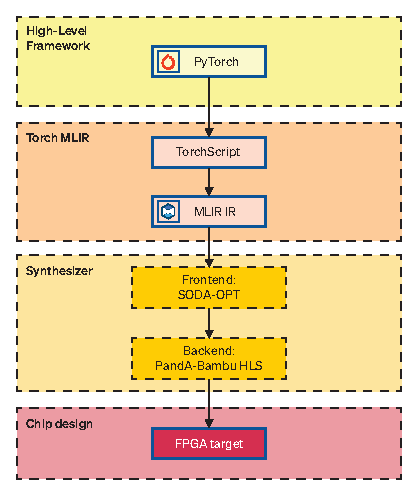
\includegraphics[height=0.6\textwidth]{Images/toolchain}
    \caption{FPGA Toolchain for Graph Neural Network Acceleration}
    \label{fig:toolchain}
\end{figure}

\section{PyTorch}
\label{sec:toolchain-pytorch}%

PyTorch~\cite{DBLP:journals/corr/abs-1912-01703} is an open-source deep learning framework widely used for building and training artificial neural networks for various machine learning tasks.

The first step of the toolchain is to design and implement the Graph Neural Network model in PyTorch.
Doing so involves defining the GNN model architecture and writing the necessary forward pass to compute node and graph-level representations.
Once having defined the model, the next step is training the GNN using standard PyTorch techniques, such as defining a loss function, setting up an optimizer, and performing backpropagation to optimize the model parameters.

\subsection{Toolchain inputs}
\label{subsec:toolchain-inputs}%

Two main models have been used as input for the developed toolchain: a Graph Isomorphism Network from OGB~\cite{NEURIPS2020_fb60d411, ogb_gnn_models}, written using PyTorch Geometric~\cite{DBLP:journals/corr/abs-1903-02428}, and a Graph Convolutional Network~\cite{DBLP:journals/corr/KipfW16, pygcn}, written using PyTorch~\cite{DBLP:journals/corr/abs-1912-01703}.

Most research and experiments have been conducted using the GCN model.
The GCN class, shown in Listing~\ref{lst:gcn-class}, is characterized by two Graph Convolutional layers, and the forward function of each layer, shown in Listing~\ref{lst:gcn-layer-forward}, is implemented through two matrix multiplications.

\begin{lstlisting}[language=Python,label={lst:gcn-class}, numbers=left, xleftmargin=2em, caption=Class of GCN model, float]
import torch.nn as nn
import torch.nn.functional as F
from pygcn.layers import GraphConvolution

class GCN(nn.Module):
    def __init__(self, nfeat, nhid, nclass, dropout):
        super(GCN, self).__init__()

        self.gc1 = GraphConvolution(nfeat, nhid)
        self.gc1 = GraphConvolution(nhid, nclass)
        self.dropout = dropout

    def forward(self, x, adj):
        x = F.relu(self.gc1(x, adj))
        x = F.dropout(x, self.dropout,
                      training=self.training)
        x = self.gc2(x, adj)
        return F.log_softmax(x, dim=1)
\end{lstlisting}


\begin{lstlisting}[language=Python,label={lst:gcn-layer-forward}, numbers=left, xleftmargin=2em, caption=Forward function of GCN layer, float]
    def forward(self, input, adj):
        support = torch.mm(input, self.weight)
        output = torch.spmm(adj, support)
        if self.bias is not None:
            return output + self.bias
        else:
            return output
\end{lstlisting}

OGB provides different datasets that can be used with their models.
The one used for this thesis is called \textit{ogbg-molhiv}, a molecular property prediction dataset.
In each graph representing a molecule, nodes correspond to atoms, and edges represent chemical bonds.
The input node features consist of nine dimensions, encompassing information like atomic number, formal charge, and whether the atom is part of a ring.
The binary classification task for GIN consists in achieving precise predictions of target molecular properties, for example, determining whether a molecule inhibits HIV replication or not.

The dataset used for the GCN model is the \textit{Cora} one.
This dataset contains 2708 scientific publications, categorized into one of seven classes.
The citation network contains 5429 links.
Each publication in the dataset is represented by a binary-valued word vector, indicating the absence or presence of the corresponding word from a dictionary of 1433 unique words.
The task is a multiclass classification, in which, given a paper, the objective is to classify it into one of the seven classes correctly.

\section{Torch-MLIR}
\label{sec:toolchain-torch_mlir}%

\begin{figure}[t]
    \centering
    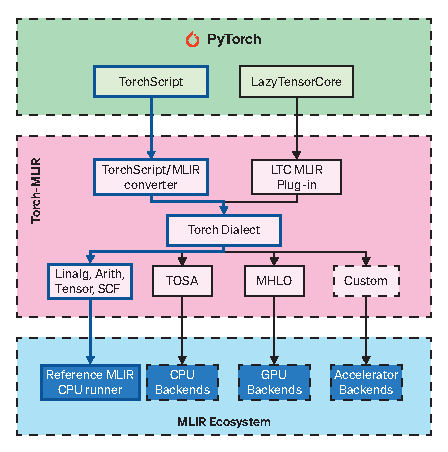
\includegraphics[height=0.6\textwidth]{Images/torch-mlir}
    \caption{Torch-MLIR flow}
    \label{fig:torch-mlir}
\end{figure}

Torch-MLIR~\cite{torch_mlir} offers compiler support for transitioning from the PyTorch ecosystem to the MLIR ecosystem.

The steps Torch-MLIR follows to go from PyTorch to MLIR are shown in Figure~\ref{fig:torch-mlir}.
In particular, the flow followed in this thesis has been highlighted with blue arrows.
There are two starting points of the flow: TorchScript and LazyTensorCode.
The one used for this research, which is also the most tested one, is TorchScript.
TorchScript~\cite{torchscript} offers a way to generate serializable and optimizable models directly from PyTorch code.

The TorchScript representation is then converted to MLIR using the built-in conversion of Torch-MLIR. The resulting MLIR IR can use different dialects that can be selected by the user, but the one used for this thesis is the Linalg dialect, which serves as input for the next phase of the toolchain.

\subsection{From PyTorch to TorchScript}
\label{subsec:pytorch-to-torchscript}%

Since Torch-MLIR implicitly uses the TorchScript representation to go from PyTorch to MLIR, the first part of the research consisted of a deep analysis of the Graph Neural Network models to make them compatible with TorchScript.

This task required more effort for the GIN model as it uses functions from PyTorch Geometric as opposed to the GCN model, which only uses pure PyTorch operations.
The following adaptations have been applied to both models, and they can be applied to make any GNN compatible with TorchScript.

\begin{itemize}
    \item[-] The GNN layer class, if created as a subclass of the Message Passing class, must be marked as Jittable whenever it is used.
\begin{lstlisting}[language=Python,label={lst:jittable}]
self.convs.append(GINConv(emb_dim).jittable())
\end{lstlisting}
    \item[-] The propagate function, if used, need its parameters to be explicitly annotated using one of the two available options: through the definition of a dictionary or through a comment.
\begin{lstlisting}[language=Python,label={lst:propagate-annotation}]
propagate_type = {'x': Tensor, 'edge_attr': Tensor}
\end{lstlisting}
\begin{lstlisting}[language=Python,label={lst:propagate-annotation-comment}]
# propagate_type: (x: Tensor, edge_attr: Tensor)
\end{lstlisting}
    \item[-] It can happen that TorchScript is not able to recognize the correct type of variables.
    In this case, it is necessary to use an assertion to explicitly declare that the variable is an instance of the correct type.
\begin{lstlisting}[language=Python,label={lst:isinstance-assertion}]
assert isinstance(edge_embedding, Tensor)
\end{lstlisting}
    \item[-] A common approach to speed up the training and inference steps is to use batched data.
    Unfortunately, TorchScript does not support forward functions that take as input a batch.
    For this reason, the forward function must receive Tensors as input, thus the batch must be split into its component.
\begin{lstlisting}[language=Python,label={lst:splitted-forward-before}]
def forward(self, batched_data):
\end{lstlisting}
\begin{lstlisting}[language=Python,label={lst:splitted-forward}]
def forward(self, x, edge_index, edge_attr):
\end{lstlisting}
    \item[-] The parameters of the forward function must be explicitly annotated with their type.
    If not declared, it is assumed to be of type Tensor.
\begin{lstlisting}[language=Python,label={lst:forward-annotation}]
def forward(self, x: Tensor, edge_index: Tensor,
            edge_attr: Tensor) -> Tensor:
\end{lstlisting}
    \item[-] TorchScript always expects an integer literal for the index, this is because indexing is only supported with integer literals.
    For this reason, cycles that do not use integer literals must be changed into enumeration.
\begin{lstlisting}[language=Python,label={lst:enumeration}]
for idx, layer in enumerate(self.convs):
\end{lstlisting}
\end{itemize}

\subsection{Torch-MLIR Compilation}
\label{subsec:torch-mlir-compilation}%

Once having designed, implemented, made compatible with TorchScript, and trained the GNN model in PyTorch, it is possible to use the \lstinline{torch_mlir.compile} API to obtain the MLIR representation of the model.
In particular, this API takes three parameters as input: the GNN model, an example input of the model and the desired output type.
The Graph Neural Network model must have been already trained, and frozen, ready for inference.
The second parameter, the example input of the model, is an arbitrary input similar to the one that would be given for inference purposes.
It is required because, by default, the implicit Jit function called by Torch-MLIR to script the model and obtain a script module involves compiling the forward method and recursively compiling any methods, submodules, and functions called within the forward method.
This results in a JIT IR which is converted to the torch dialect, which is almost in a 1:1 correspondence.
The torch dialect is then lowered into one of the three available output dialects: linalg, tosa, mhlo.
The purpose of the last parameter of \lstinline{torch_mlir.compile} is to choose which of these three dialects has to be used for the output MLIR\@.

An additional parameter that can be used is related to the tracing.
There are two ways in which it is possible to obtain a TorchScript representation: \lstinline{torch.jit.script} and \lstinline{torch.jit.trace}.
The compile API of Torch-MLIR uses the first one by default.
Instead, if the option use tracing is set to True, JIT tracing is used.
The behavior of the two functions is slightly different.

Tracing traces the execution of the code for the given inputs to generate a TorchScript representation.
It only captures functions and modules that lack untracked external dependencies (e.g., perform input/output or access global variables).
Tracing exclusively captures operations performed when the specified function is executed with the provided tensors.
Consequently, the resulting ScriptModule will consistently execute the same traced graph for any input.

In conclusion, tracing can be a valid option in some cases, such as when there is no need to record any control-flow like if-statements or loops, but the scripting is preferred, and it is guaranteed to work in a more wide set of cases.
A call example of the compile Python API of Torch-MLIR is reported below.
\begin{lstlisting}[language=Python,label={lst:torch_mlir-compile}]
module = torch_mlir.compile(gnn_model, (x, features, adj),
                            output_type="linalg-on-tensors")
\end{lstlisting}

Once having obtained the compiled module, the expected behavior is to use one of the backends provided by torch-MLIR to run inference.
This is not the flow followed in this thesis, because, as represented in the accelerator design flow in Figure~\ref{fig:toolchain}, it is time to export the Linalg representation for the next phase.
This can be done by simply saving the model to an MLIR file, as shown below.
\begin{lstlisting}[language=Python,label={lst:torch_mlir-export}]
with open("gnn_model.mlir", "w", encoding="utf-8") as outf:
    outf.write(str(module))
\end{lstlisting}

Only the GCN model implemented in PyTorch reached this phase of the toolchain.
During the research, much effort has been spent in trying to add support for the PyTorch Geometric framework to the toolchain.
Even if some improvements have been achieved in this regard, such as the implementation of support of the constant of Tuple type, there are still open points to work on.
For this reason, at the actual state, the proposed design flow only supports PyTorch as a high-level framework
In particular, Torch-MLIR does not support the \lstinline{aten.scatter_add} operation, which, at the actual state, cannot be lowered to MLIR\@.
This operation is extensively used by PyTorch Geometric, leading to the incompatibility of the two tools.

Another current limitation of the framework derives from the fact that Torch-MLIR does not support the sparse tensor type.
Each sparse tensor implemented in PyTorch, with the relative sparse operations, is lowered to MLIR to a dense tensor, losing all its representation's advantages.
A promising option to avoid this is Taco~\cite{taco} with its PyTaco APIs for Python.
MLIR-PyTACO~\cite{mlir-pytaco} is an end-to-end use case for the sparse tensor compiler, which employs a Python interface to process the PyTACO language, creating MLIR \lstinline{linalg.generic} operations annotated with sparse tensor information to depict tensor computations.
It subsequently invokes the MLIR sparse tensor code generator to produce an executable program, which is executed by the MLIR execution engine, returning the result back to the Python layer.
It is important to clarify that, as introduced in~\cite{Bik_2022}, sparse tensors are supported by MLIR, with a dedicated sparse tensor dialect that uses intuitive annotations for different sparse tensor representations, such as CSR and COO.
What is not supported yet is the lowering through Torch-MLIR\@.
However, even if MLIR-PyTACO is still premature and in testing phase, interesting features could be brought by its advancement.
In fact, part of this work successfully exported the MLIR of a sparse matrix multiplication generated by MLIR-PyTACO\@.
It has been then used as input for the sparse compiler to obtain the LLVM representation, which could be synthesized using PandA-Bambu with additional development time to support some constructs that are currently incompatible with PandA-Bambu.

Even without the sparse tensor representation, using the proper optimizations provided by the toolchain in combination with the higher computational performance of FPGAs, still makes it possible to accelerate the GNN operations, as will be stated in the next Chapter.

\section{Synthesizer}
\label{sec:toolchain-synthesizer}%

The synthesizer represents the final step of the toolchain, which optimizes and synthesizes the MLIR representation, targeting FPGA\@.
This step includes SODA-OPT and PandA-Bambu, both introduced in Section~\ref{sec:soda}.
The following Subsections provide insight into what is happening internally to these two components.

\begin{figure}[t]
    \centering
    \subfloat[Compiler frontend\label{fig:soda-opt_flow}]{
        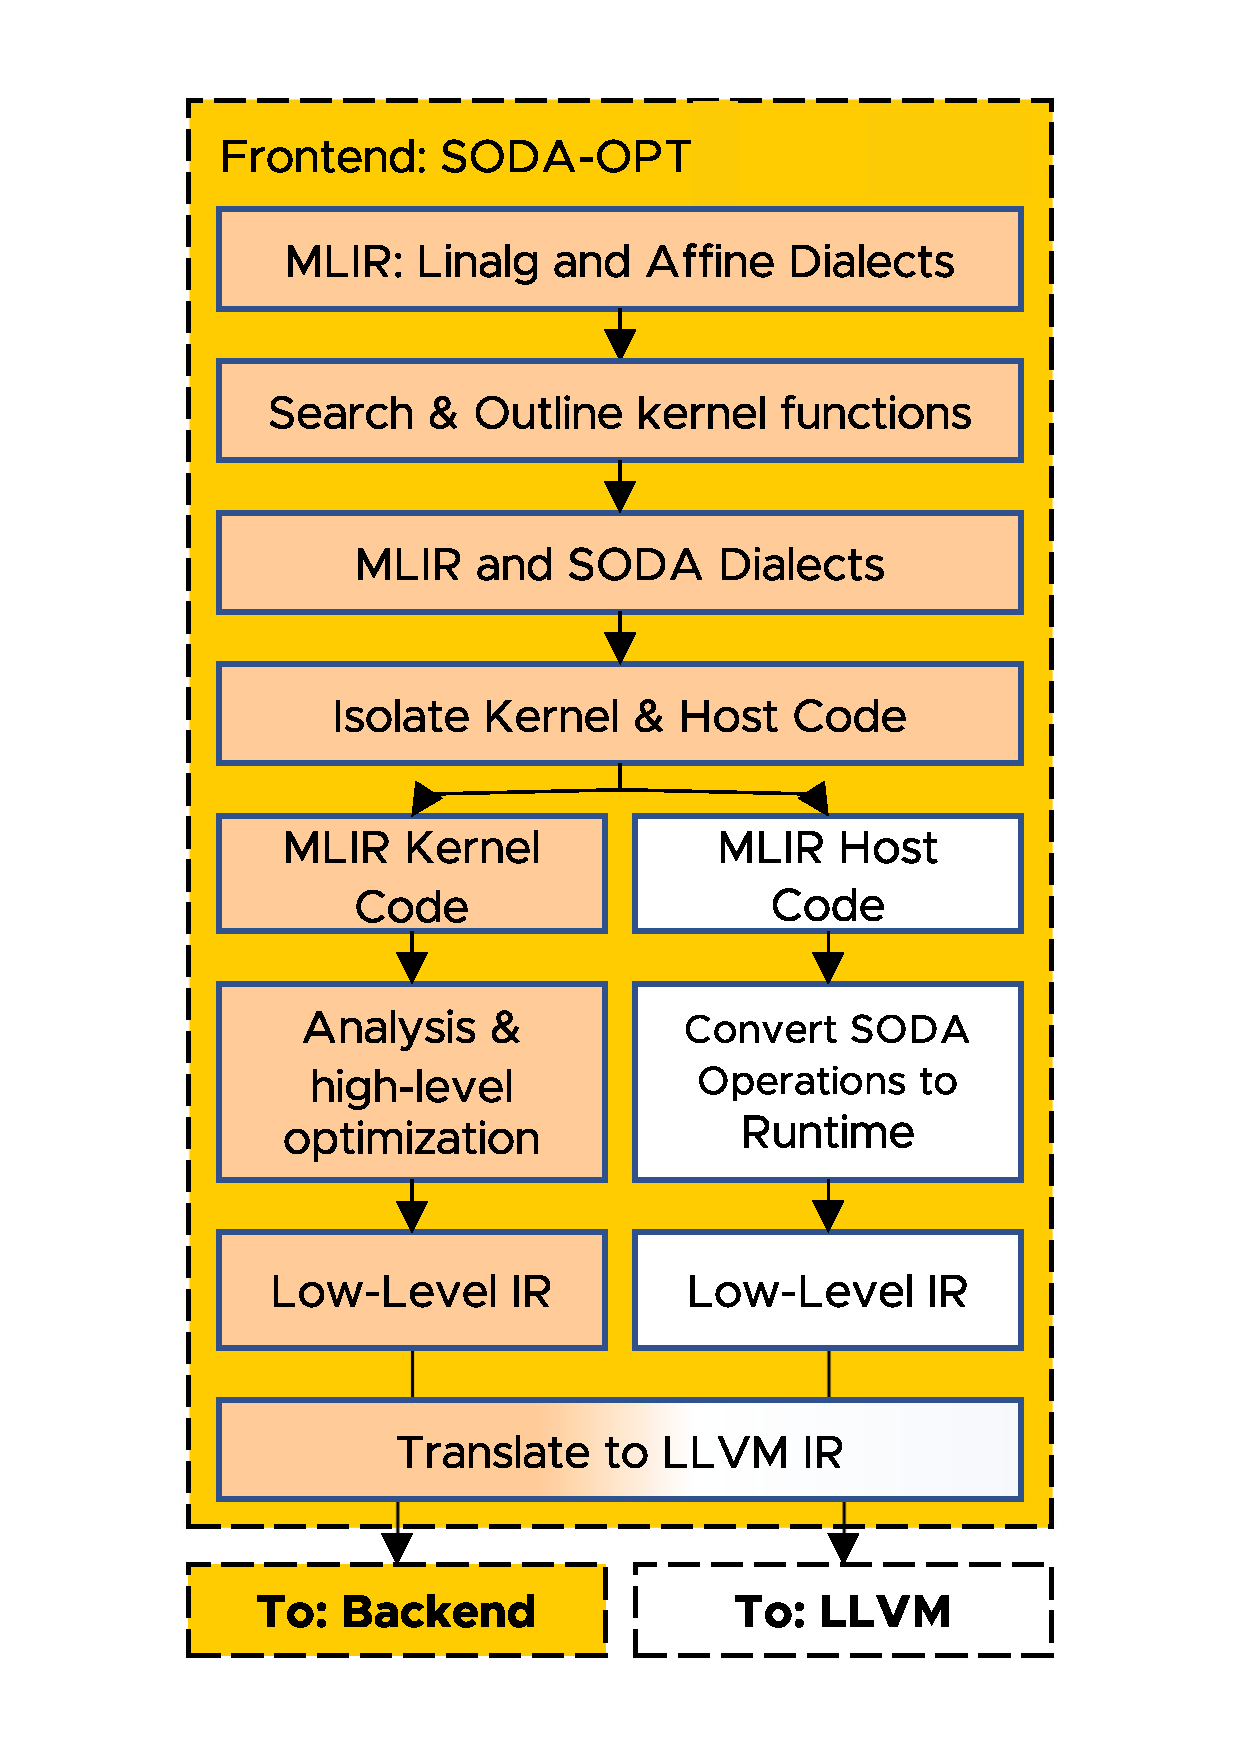
\includegraphics[height=0.6\textwidth]{Images/soda_opt_flow}
    }
    %\quad
    \hspace{0.03\textwidth}
    \subfloat[High-level synthesis backend\label{fig:bambu_flow}]{
        \captionsetup{width=.4\textwidth}
        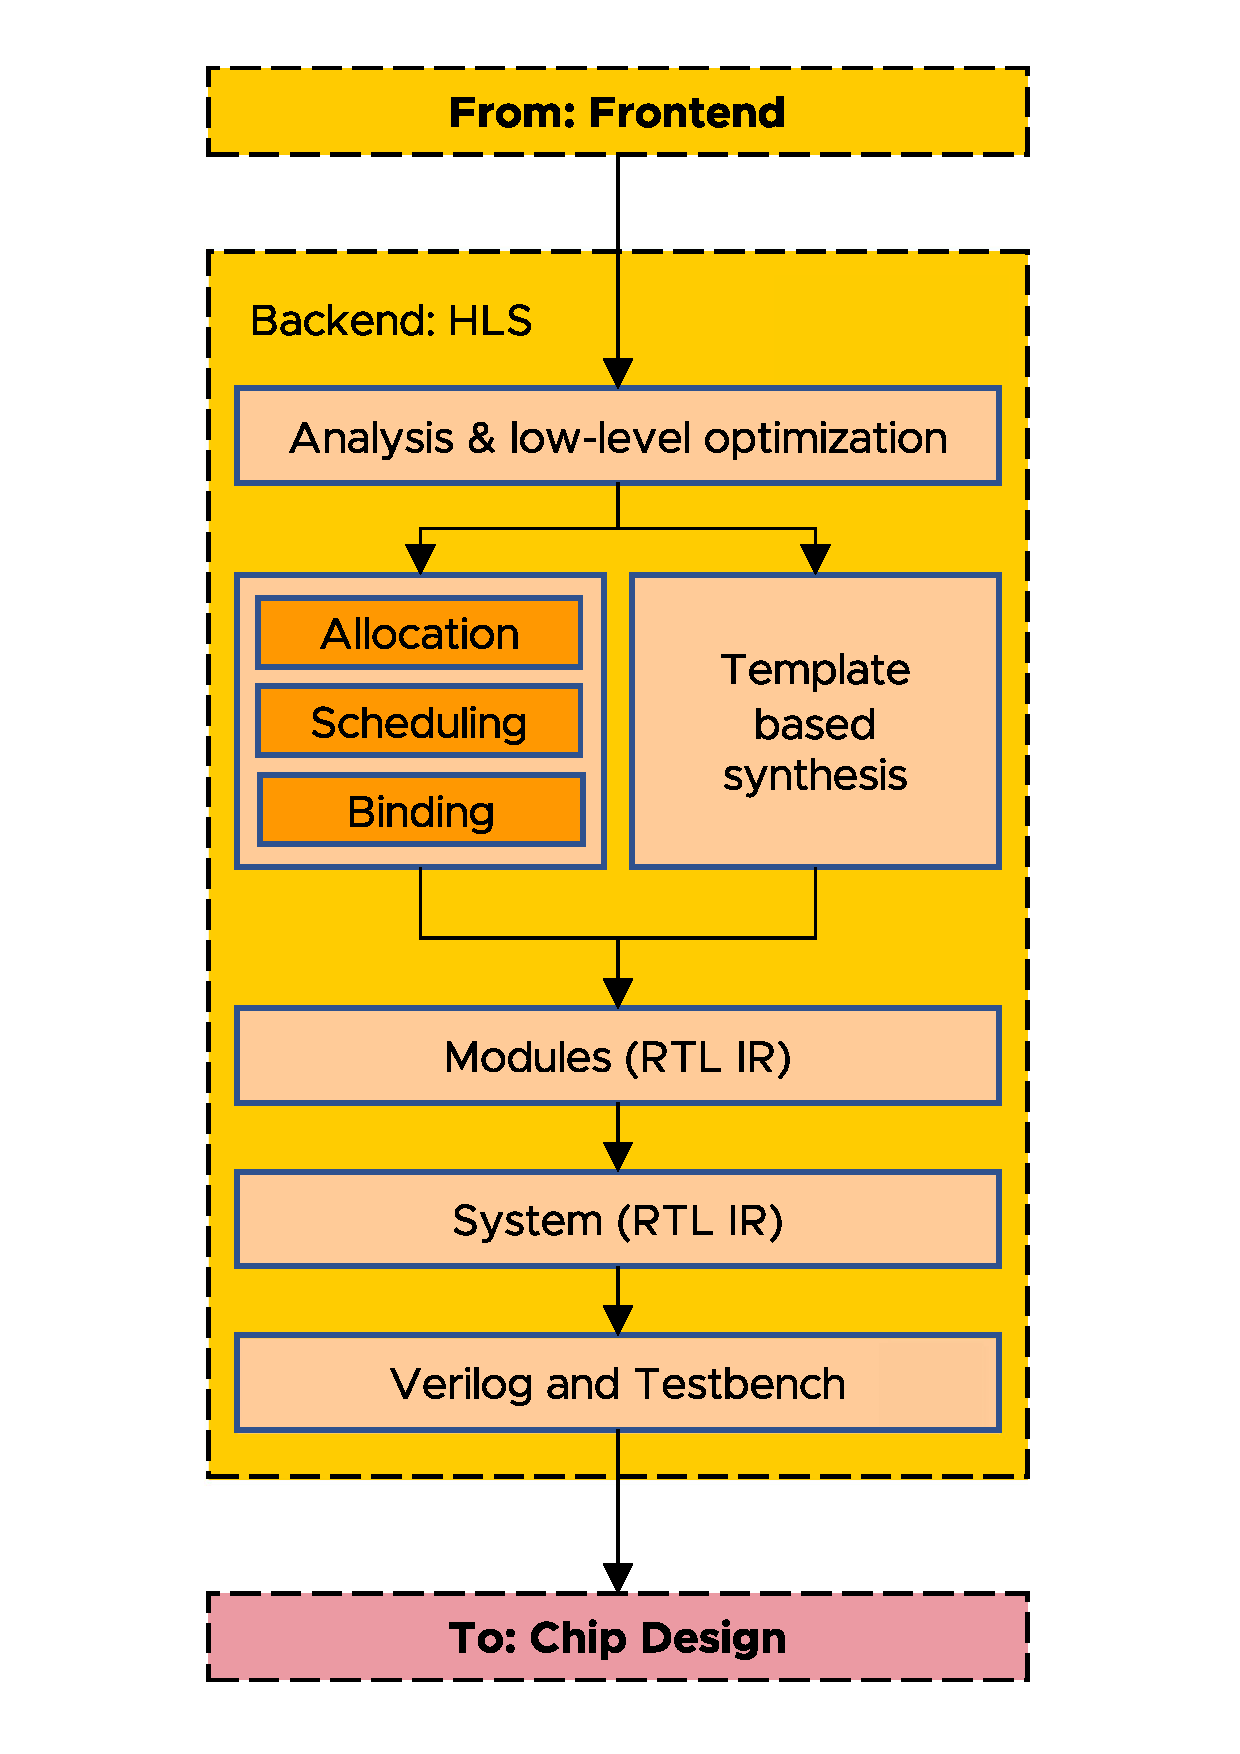
\includegraphics[height=0.6\textwidth]{Images/bambu_flow}
    }
    \caption{Synthesizer: SODA-OPT and PandA-Bambu overview~\cite{9786533}}
    \label{fig:synthesizer_flow}
\end{figure}

\subsection{SODA-OPT}
\label{subsec:toolchain-soda_opt}%

SODA-OPT, as shown in Figure~\ref{fig:soda-opt_flow}, receives as input the MLIR representation of the model.
This step is primarily responsible for applying optimizations that can be exploited in the next step.
In particular, a subset of MLIR passes can be used to do so.
The output of SODA-OPT is an LLVM representation that serves as input to PandA-Bambu HLS\@.

Despite the remarkable capabilities of SODA-OPT, it should be noted that it does not support the entire set of dialects utilized within the MLIR ecosystem, such as the ml\_program or the Tensor dialect.
Consequently, an additional step is required wherein the representation obtained from Torch-MLIR is lowered to remove unsupported dialects.
In particular, once having successfully exported the MLIR representation using the \lstinline{torch_mlir.compile} API, a set of mlir-opt passes have been used to remove the unsupported dialects by lowering them to supported ones, such as memref.

The next step consists in outlining the part of MLIR code to accelerate.
In general, the aim is to accelerate the whole function.
To do so, it is enough to modify the MLIR file by adding \lstinline{soda.launch} and \lstinline{soda.terminator} flags at the beginning and end of the function, thus after the start of the forward method and before the return statement.

SODA-OPT provides various passes that can be used to apply optimization to the outlined code.
In particular, it provides a subset of MLIR passes and a set of custom passes.
The SODA-OPT passes are continuously evolving, trying to keep up with rapid advancement and innovation within the domain of MLIR\@.

SODA-OPT, after having identified the key code regions, having outlined them into separate MLIR modules, and having applied the transformation passes to the MLIR input, optimizes the portion of code selected for hardware acceleration with a progressive lowering through different MLIR dialects.
As a final result, the input code is translated into an LLVM intermediate representation intentionally restructured for hardware synthesis.

\subsection{PandA-Bambu}
\label{subsec:toolchain-panda_bambu}%

PandA-Bambu represents the last phase of the synthesis.
As represented in Figure~\ref{fig:bambu_flow}, it receives the LLVM representation as input, and after having applied some optional low-level optimizations, it performs the typical steps of HLS introduced in Section~\ref{sec:hls}.

The LLVM intermediate representation taken as input from PandA-Bambu is received by the Clang compiler frontend which builds an internal IR to perform the HLS steps.
After having applied the specified optimizations, the generated design in an HDL is given as output.
As a result, after traversing through each stage of the proposed toolchain's process, PandA-Bambu's output represents the final output, an accelerator tailored to target and maximize performance on cutting-edge FPGA architectures.

PandA-Bambu allows the specification of different optimizations and settings that can have a big impact on accelerator performance.
Some optimization techniques have been explored, including in particular an evaluation of the impact of varying the number of memory channels.

In particular, an experimental analysis has been performed varying the number of memory channels, between the minimum, 2 channels, and the maximum, 32 channels.
The latter option uses an external memory for the accelerator, which allows to better exploit the high level of parallelism that can be achieved using the loop unrolling technique, but at the same time, more cycles and area for loading data are required.
It is the case of a trade-off between the number of channels and the required number of data load cycles.
The conducted study revealed that there is a point, represented by a specific number of parallel operations, after which using an external memory with 32 channels becomes beneficial.

PandA-Bambu also offers the possibility to apply low-level loop unrolling, but this option has been disabled to be able to evaluate in isolation the performance impact of the SODA-OPT loop unrolling technique and avoid that loops are unrolled automatically if the option was not enabled in SODA-OPT\@.
PandA-Bambu provides also the possibility to export some files that have been used for this research.
One important file is represented by the HLS graph, which shows the computation states and transitions, the number of cycles needed by each operation to complete, and other information that has been useful to study and understand the impact of both SODA-OPT and PandA-Bambu optimization settings.

\section{Matrix multiplication acceleration}
\label{sec:matmul-algo}%

An essential part of this research has been the analysis of the GNN model, the understanding of its bottlenecks, and the consequent identification of the optimization having the biggest impact on performance, without increasing too much the area of the accelerator.

The first part of this analysis has been conducted on PyTorch.
Profiling the inference function of the GCN model, the result showed that, in general, nearly 60\% of the time required to make a prediction was used for the matrix multiplication operation as will be shown in Chapter~\ref{ch:chapter_six}.
For this reason, an important part of this thesis is represented by research on how to optimize matrix multiplication using SODA-OPT passes to then accelerate the GCN inference.

\begin{algorithm}[t]
    \label{alg:matmul_pseudo}
    \caption{Naive matrix multiplication algorithm}
    \label{alg:var}
    \label{protocol1}
    \begin{algorithmic}[1]
    \STATE \textbf{Data:} $A[R][P], B[M][N]$
    \STATE \textbf{Result:} $C[R][N]$
    \IF{$P == M$}
    \FOR{$m=0; m<R, m++$}
    \FOR{$r=0; r<N, r++$}
    \STATE $C[m][r] = 0$
    \FOR{$k=0; k<M, k++$}
    \STATE $C[m][r] += A[m][k] * B[k][r]$
    \ENDFOR
    \ENDFOR
    \ENDFOR
    \ENDIF
    \end{algorithmic}
\end{algorithm}

The naive implementation of the row-by-column multiplication, whose pseudocode is shown in Algorithm~\ref{alg:var}, is characterized by three nested loops.
The multiplication is possible only in the case the number of column of the first matrix is equal to the number of row of the second one.
Figure~\ref{fig:row-by-col-mul-example} highlight how an element of the output matrix is computed, using a row of the first matrix and a column of the second one.
In a general matrix multiplication, shown in Equation~\ref{eq:matmul}, each element of the new matrix can be computed accordingly to Equation~\ref{eq:matmul-element}.

\begin{equation}
        \label{eq:matmul}
    \begin{pmatrix}
     a_{11} & a_{12} & \cdots & a_{1n}\\
     a_{21} & a_{22} & \cdots & a_{2n}\\
     \vdots & \vdots & \ddots & \vdots\\
     a_{m1} & a_{m2} & \cdots & a_{mn}
 \end{pmatrix}
 \times
 \begin{pmatrix}
     b_{11} & b_{12} & \cdots & b_{1p}\\
     b_{21} & b_{22} & \cdots & b_{2p}\\
     \vdots & \vdots & \ddots & \vdots\\
     b_{n1} & b_{n2} & \cdots & b_{np}
 \end{pmatrix}
  =
 \begin{pmatrix}
     c_{11} & c_{12} & \cdots & c_{1p}\\
     c_{21} & c_{22} & \cdots & c_{2p}\\
     \vdots & \vdots & \ddots & \vdots\\
     c_{m1} & c_{m2} & \cdots & c_{mp}
 \end{pmatrix}
\end{equation}

\begin{equation}
    \label{eq:matmul-element}
    c_{ij}= a_{i1} b_{1j} + a_{i2} b_{2j} +\cdots+ a_{in} b_{nj} = \sum_{k=1}^n a_{ik}b_{kj}
\end{equation}

\begin{figure}[t!]
    \centering
    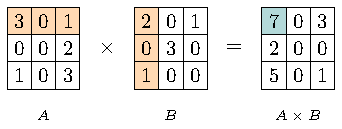
\includegraphics[height=0.24\textwidth]{Images/row-by-col-mult-example}
    \caption{Row-by-column matrix multiplication example}
    \label{fig:row-by-col-mul-example}
\end{figure}

A matmul operation in the linalg dialect lowered to affine by SODA-OPT results in three nested affine loops shown in Listing~\ref{lst:affine-mul}.

Among all optimizations available in SODA-OPT the biggest improvement in terms of performance is achieved applying the loop unrolling technique, which involves expanding completely or partially the loop, effectively reducing the overhead of loop control instructions and potentially exposing more opportunities for other optimizations.
There are two available options: full unrolling and partial unrolling.
In the former the entire loop is expanded until the loop is completely removed, resulting in a significant increase in the size of the code.
In the latter, instead, only a subset of the loop iterations is expanded into multiple iterations.
A parameter, called \textit{unroll factor}, can be set to decide the number of loop iterations that are combined into a single iteration.
Listing~\ref{lst:affine-mul-unroll3} shows the effect of a partial unrolling, with unrolling factor equal to 5, to the matrix multiplication introduced in Listing~\ref{lst:affine-mul}.

The loop unrolling technique perfectly allows to exploit the extreme parallelism available on FPGAs, because the loop bodies are expanded allowing the parallel execution of multiple iterations of the original loop.
The right choice is not to continuously unroll until having no more loops in the code.
The solution is to pick the right trade-off between performance reduction and area consumption.

The number of cycles needed by an accelerator generated by PandA-Bambu without loop unrolling can be calculated using Equation~\ref{eq:number-cycles}.
The notation used refers to Equation~\ref{eq:matmul}, but it can be referred to Algorithm~\ref{alg:var} by considering $n = M \land m=R \land p=N$.
The first part of the equation computes the total number of iterations, while the second half computes the number of cycles needed to perform multiplications and additions, and to load and store data.
The number of cycles needed to load and store data are computed by adding one cycle for each $ch$ operands read, and one cycle for each $ch$ operand written, with $ch$ equal to the number of memory channels.
From Listing~\ref{lst:affine-mul}, it can be seen that there are three load and one store, for a total of four memory operations.

\begin{lstlisting}[label={lst:affine-mul}, caption=Matrix multiplication in MLIR affine dialect, float]
affine.for %arg3 = 0 to 15 {
  affine.for %arg4 = 0 to 16 {
    affine.for %arg5 = 0 to 15 {
    %0 = affine.load %arg0[%arg3, %arg5] : memref<15x15xf32>
    %1 = affine.load %arg1[%arg5, %arg4] : memref<15x16xf32>
    %2 = affine.load %arg2[%arg3, %arg4] : memref<15x16xf32>
    %3 = arith.mulf %0, %1 : f32
    %4 = arith.addf %2, %3 : f32
    affine.store %4, %arg2[%arg3, %arg4] : memref<15x16xf32>
    }
  }
}
\end{lstlisting}

\begin{equation}
    \label{eq:number-cycles}
    cycles = \left(  n \cdot m \cdot p \right) \cdot \left(  cycles_{mul} + cycles_{add} + \frac{4}{ch} \right)
\end{equation}

Let us consider two matrices, the first of size $15\times15$ and the second of size $15\times16$.
The FPGA model used for the experimental phase uses three cycles for floating-point addition and two cycles for floating-point multiplication, both single precision.
By applying the Equation~\ref{eq:number-cycles}, the expected number of cycles for computing such matrix multiplication, using two memory channels is 25,200.

\begin{lstlisting}[label={lst:affine-mul-unroll3}, caption=Unrolled matrix multiplication in affine dialect with unrolling factor 5, float]
affine.for %arg3 = 0 to 15 {
  affine.for %arg4 = 0 to 16 {
    affine.for %arg5 = 0 to 15 step 5 {
      %0 = affine.load %arg0[%arg3, %arg5] : memref<15x15xf32>
      %1 = affine.load %arg1[%arg5, %arg4] : memref<15x16xf32>
      %2 = affine.load %arg2[%arg3, %arg4] : memref<15x16xf32>
      %3 = arith.mulf %0, %1 : f32
      %4 = arith.addf %2, %3 : f32
      affine.store %4, %arg2[%arg3, %arg4] : memref<15x16xf32>
      %5 = affine.apply affine_map<(d0) -> (d0 + 1)>(%arg5)
      %6 = affine.load %arg0[%arg3, %5] : memref<15x15xf32>
      %7 = affine.load %arg1[%5, %arg4] : memref<15x16xf32>
      %8 = affine.load %arg2[%arg3, %arg4] : memref<15x16xf32>
      %9 = arith.mulf %6, %7 : f32
      %10 = arith.addf %8, %9 : f32
      affine.store %10, %arg2[%arg3, %arg4] : memref<15x16xf32>
      %11 = affine.apply affine_map<(d0) -> (d0 + 2)>(%arg5)
      %12 = affine.load %arg0[%arg3, %11] : memref<15x15xf32>
      %13 = affine.load %arg1[%11, %arg4] : memref<15x16xf32>
      %14 = affine.load %arg2[%arg3, %arg4] : memref<15x16xf32>
      %15 = arith.mulf %12, %13 : f32
      %16 = arith.addf %14, %15 : f32
      affine.store %16, %arg2[%arg3, %arg4] : memref<15x16xf32>
      %17 = affine.apply affine_map<(d0) -> (d0 + 3)>(%arg5)
      %18 = affine.load %arg0[%arg3, %17] : memref<15x15xf32>
      %19 = affine.load %arg1[%17, %arg4] : memref<15x16xf32>
      %20 = affine.load %arg2[%arg3, %arg4] : memref<15x16xf32>
      %21 = arith.mulf %18, %19 : f32
      %22 = arith.addf %20, %21 : f32
      affine.store %22, %arg2[%arg3, %arg4] : memref<15x16xf32>
      %23 = affine.apply affine_map<(d0) -> (d0 + 4)>(%arg5)
      %24 = affine.load %arg0[%arg3, %23] : memref<15x15xf32>
      %25 = affine.load %arg1[%23, %arg4] : memref<15x16xf32>
      %26 = affine.load %arg2[%arg3, %arg4] : memref<15x16xf32>
      %27 = arith.mulf %24, %25 : f32
      %28 = arith.addf %26, %27 : f32
      affine.store %28, %arg2[%arg3, %arg4] : memref<15x16xf32>
    }
  }
}
\end{lstlisting}

This heuristic served as a guide to better understand which optimizations might be most appropriate and would yield the most significant positive impact on performance.

%\subsection{Emulating global memory coalescing of CUDA}
%\label{subsec:CUDA-coalescing}%
%
%The work in~\cite{opt_cuda_matmul} iteratively optimize an implementation of matrix multiplication written in CUDA, and it is a useful resource to understand which techniques can be applied also to FPGAs.
%One of the most interesting optimizations that this work tried to apply to FPGA architecture is global memory coalescing, a memory optimization technique employed in parallel computing, specifically within the context of GPU programming and CUDA\@.
%Its objective is to enhance the efficiency of memory access patterns and data transfers when multiple threads or processing units concurrently access global memory.
%This is accomplished through the reduction of memory access latency and bandwidth consumption, organizing memory accesses in a manner that optimizes the utilization of the memory hierarchy and the bus bandwidth of GPUs and similar parallel processors.
%During execution, the threads within a block are organized into entities known as warps, which are subsequently allocated to warp schedulers, i.e.\ the physical cores responsible for executing instructions.
%Each multiprocessor houses four warp schedulers and each warp comprises 32 threads.
%The arrangement into warps is determined by a value called threadId in a consecutive sequence, ensuring that threads with neighboring threadId values are grouped together within the same warp.
%
%\begin{figure}[t!]
%    \centering
%    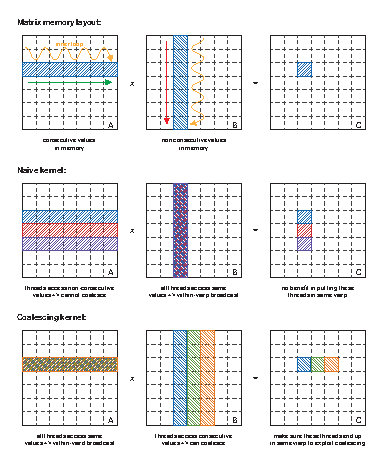
\includegraphics[height=0.8\textwidth]{Images/memory-coalescing}
%    \caption{Matrix multiplication memory coalescing~\cite{opt_cuda_matmul}}
%    \label{fig:memory-coalescing}
%\end{figure}
%
%The author of this work enables coalescing changing how positions of the result matrix C are assigned to threads.
%This change in the global memory access pattern is illustrated in Figure~\ref{fig:memory-coalescing}.
%
%To reproduce the behaviour of the coalescing kernel shown in Figure~\ref{fig:memory-coalescing}, multiple memory channels has been used.
%Using burst read and write operations allows for transferring multiple data elements in a single memory access, enhancing memory coalescing.
%This optimization enriched the structure of the accelerator, by loading and storing multiple data in parallel and thus using more PEs  in parallel to perform operations such as multiplications and additions.

\section{Conclusion}
\label{sec:toolchain-discussion}%

This chapter presented the main contribution of this thesis, an FPGA toolchain to create GNN hardware accelerators starting directly from PyTorch high-level framework, with the possibility to use different optimizations to improve performance depending on application bottlenecks.

The most crucial advantage of the proposed toolchain is that it allows obtaining an accelerator without any knowledge of hardware design and implementation.

Furthermore, an examination of two representative GNN models has revealed that a significant portion of the computational workload consists of matrix multiplication operations.
The following chapter provides experimental evidence demonstrating the impact of using tailored optimization passes in SODA-OPT and PandA-Bambu specifically for matrix multiplication.